\chapter{\textit{Lean Startup}}


\section{¿Qué es una \textit{Startup}?}
Una \textit{startup} es una institución humana  diseñada para crear un nuevo producto o servicio bajo condiciones de incertidumbre extrema.


Es precisamente esa incertidumbre extrema la que hace que una \textit{startup} no se pueda gestionar con los mismos métodos y estándares que utilizan las empresas consolidadas. Tampoco las nociones de éxito o fracaso son lo mismo en ambos ámbitos, porque una startup necesita del fracaso y el aprendizaje continuos como mecanismos para evaluar sus hipótesis de partida.


\section{El método \textit{Lean Startup}}
El método \textit{Lean Startup} es un conjunto de prácticas pensadas para ayudar a los emprendedores a incrementar las probabilidades de crear una \textit{startup} con éxito. 


El método \textit{Lean Startup} está diseñado para enseñar a conducir a una startup a través de la experimentación. En lugar de hacer planes complejos basados en muchas asunciones, se pueden hacer ajustes constantes mediante un ciclo de \textit{feedback} constante de Crear-Medir-Aprender (ver figura \ref{fig:lean_startup}). A través de este proceso de dirección, podemos aprender cómo saber si ha llegado el momento de hacer un giro drástico llamado pivote o si debemos perseverar en nuestra trayectoria actual. Cada contratiempo es una oportunidad para aprender cómo llegar al punto donde queremos ir (conocimiento validado). Lo importante es llegar a tu destino sin importar los caminos que tomes. Este destino se trata de crear un negocio próspero que cambie el mundo.


\subsection{Crear}
El esfuerzo de una \textit{startup} está en realizar experimentos que prueben nuestras estrategias. Estos experimentos siguen el método científico: Empiezan con unas hipótesis que hacen predicciones sobre lo que supestamente pasa. Entonces, se prueba empíricamente estas predicciones sobre consumidores reales y lo más rápido posible consumiendo el mínimo esfuerzo.


Para medir empíricamente nuestras hipótesis, se desarrolla un producto mínimo viable, en adelante PMV, con la finalidad de comprobar que esas hipótesis que se mantienen en el tiempo son realmente ciertas. Pero no hay que fiarse completamente de la opinión del cliente, puesto que muchas veces ni él mismo sabe lo que quiere o necesita.


\subsection{Medir}
Se necesita un enfoque disciplinado y sistemático para saver si estamos progresando y descubrir si estamos obteniendo aprendizaje validado. Este sistema es la contabilidad de la innovación que funciona en tres etapas:
\begin{enumerate}
\item \textit{Primera etapa: } Un PMV permite a una \textit{startup} obtener datos reales sobre el punto de partida; y esto es valioso como base para el aprendizaje sobre los consumidores y sus reacciones al producto incluso aunque empiece con unas noticias extremadamente malas. Cuando uno escoge entre las muchas asunciones de un plan de negocio, tiene sentido probar primero las más arriesgadas. Si no puede mitigar estos riesgos para llegar al ideal que se requiere para un negocio sostenible, no tiene sentido probar lo demás.
\item \textit{Segunda etapa: } Cada iniciativa de desarrollo de producto, de marketing o de cualquier otra actividad que lleve a cabo una \textit{startup} debería tener el objetivo de mejorar uno de los factores clave del modelo de crecimiento.
\item \textit{Tercera etapa: } Con el tiempo, un equipo que está aprendiendo cuál es su camino hacia un negocio sostenible verá que las cifras de su modelo aumentan desde los niveles horribles del punto de partida establecido por el PMV y convergen hacia algo similar al ideal del plan de negocio. Una startup que fracasa en este aspecto verá que el ideal se aleja cada vez más, y debe pivotar.
\end{enumerate}


\subsection{Aprender}
Si no estamos haciendo progresos suficientes como para creer que nuestra hipótesis estratégica inicial es correcta y debemos hacer un gran cambio, a este cambio se le llama pivotar. Un pivote es una corrección estructurada diseñada para probar una nueva hipótesis básica sobre el producto, la estrategia y el motor de crecimiento.


No hay mayor destrucción del potencial creativo que la decisión errónea de perseverar. Las empresas que no pueden pivotar hacia una nueva dirección a partir del feedback recibido del mercado se pueden quedar atascadas, sin crecer lo suficiente ni morir, consumiendo los recursos y el compromiso de los empleados y accionistas pero sin avanzar\cite{ericries2011}.

\begin{figure}[htbp] 
    \centering
    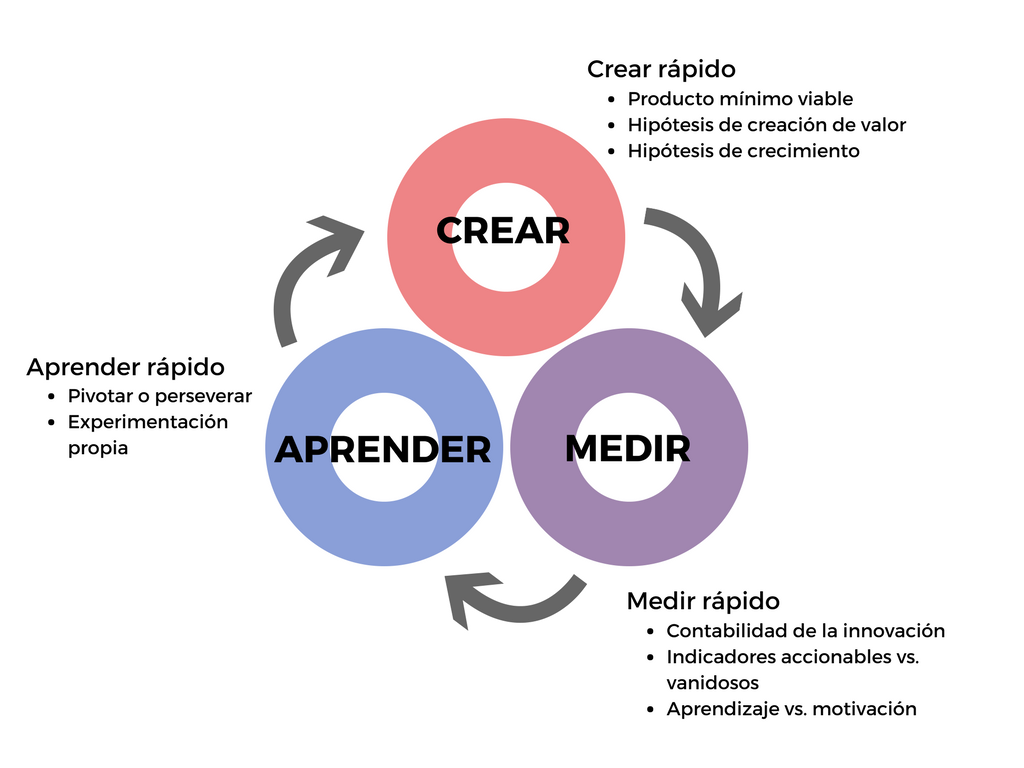
\includegraphics[width=1\textwidth]{figuras/lean_startup.png}
    \caption{Metodología \textit{Lean Startup}}
    \label{fig:lean_startup}
\end{figure}	


%La mayoría de herramientas del management tradicional no están diseñadas para prosperar en el duro suelo de incertidumbre extrema en que crecen las startups. El futuro es impredecible, los consumidores disponen de una creciente gama de alternativas y el ritmo del cambio se acelera constantemente.

